\begin{figure}[h]
    \centering
    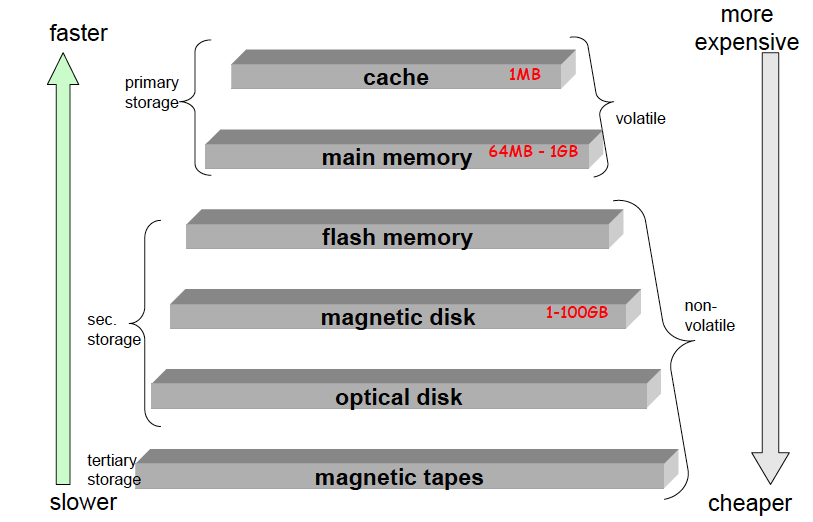
\includegraphics[width=0.8\textwidth, keepaspectratio]{GerarchieMemorie.png}
    \label{fig:memorie}
\end{figure}

\subsection{Prestazioni}
$$\text{tempo di accesso} = \text{latenza} + \frac{\text{dimensione dati da trasferire}}{\text{velocità di trasferimento}}$$
Dove la \textbf{latenza} \`e il tempo necessario ad accede al primo byte, e il \textbf{tempo di trasferimento} \`e il tempo necessario a muovere i dati\\
\textbf{Tempo di latenza}: tempo impiegato per raggiungere le informazioni di interesse.\\
Il tempo di latenza \`e composto da:
\begin{itemize}
    \item \textbf{Command overhead time}: Tempo per impartire i comandi al drive (trascurabile, intorno a $0.5$ msec)
    \item \textbf{Seek Time} (Ts): Tempo impiegato dal braccio a posizionarsi sulla traccia desiderata. Tempo medio $2-10$ msec, tempo massimo $2-20$ msec
    \item \textbf{Settle Time}: Tempo richiesto per la stabilizzazione del braccio
    \item \textbf{Rotational Latency} (Tr): Tempo di attesa del primo settore da leggere. $2-11$ msec
\end{itemize}
$$\text{Tempo di trasferimento} = \frac{(\text{bytes}/\text{sector}) \times (\text{sectors}/\text{track})}{\text{rotational time}}$$
Conversione RPM in \textit{rotational time}:
$$7200 \text{ rpm } (\text{rounds per minute})= \frac{1}{7200} \text{minutes}/\text{round} =$$
$$ \frac{60}{7200} \text{seconds per round} (\text{rotational time})$$

\subsection{Blocchi o Pagine}
Hanno una dimensione di qualche KB ($4-64 \text{KB}$).\\
\textbf{Un blocco} (o pagina) è una sequenza contigua di settori su una traccia, e costituisce l'unità di I/O per il trasferimento di dati da/per la memoria principale.\\
Tempo di trasferimento: $1 \text{msec}$ per blocchi da $4 \text{KB}$

\subsection{Struttura dei File}
Ogni file ha una dimensione fissa e contiene un numero arbitrario di tuple.\\
Le tuple (record) vengono salvate con i campi a dimensione non variabile prima, e quelli a dimensione variabile dopo. All'inizio del record, per ogni campo a lunghezza variabile abbiamo un "prefix pointer" che indica il primo byte del campo.\\
In generale, ogni record contiene un \textbf{header} che contiene:
\begin{itemize}
    \item La lunghezza del record
    \item L'identificatore della relazione al quale appartiene
    \item L'identificatore univoco del record nel DB
    \item Un timestamp che indica quando il record \`e stato inserito o modificato l'ultima volta
\end{itemize}
I record vengono inseriti a partire dal "fondo" del file e salendo.\\
Ogni file inizia con un "Page header" che contiene informazioni queli:
\begin{itemize}
    \item ID della pagina nel DB (PID)
    \item timestamp dell'ultima modifica
    \item relazione di appartenenza
    \item altro
\end{itemize}

\begin{figure}[h]
    \centering
    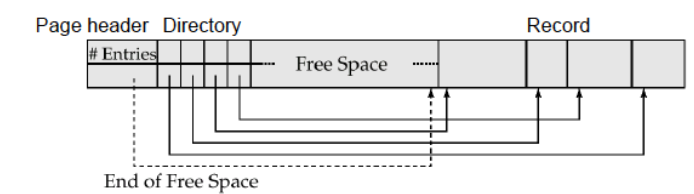
\includegraphics[width=0.8\textwidth, keepaspectratio]{strutturaFile.png}
    \label{fig:file}
\end{figure}

\noindent
\textbf{L'organizzazione} dei blocchi su disco viene gestita tramite l'uso di \textbf{bucket} cioè un insieme di blocchi, non necessariamente contigui ma "vicini", possibilmente nello stesso cilindro, dove salviamo record tra loro collegati.

\break
\subsection{Tipi di file}
\begin{itemize}
    \item \textbf{File heap}: Ordine di inserimento
    \item \textbf{File ordinato}: Ordinati secondo uno o più campi
    \item \textbf{File Hash}: record che hanno lo stesso valore per un campo sono memorizzati vicini
\end{itemize}
L'organizzazione a seconda dei campi in tuple "contigue" in memoria \`e detta \textbf{clustering} ed \`e legata all'uso degli indici (indici clusterizzati).
Il \textbf{co-clustering} invece riguarda pagine con tuple provenienti da più relazioni clusterizzate nella stessa pagina (utili per il join o operazioni simili).

\subsection{Buffer}
Il buffer \`e organizzato in pagine della stessa dimensione delle pagine/blocchi su disco.\\
Utilizza policy diverse dai Sistemi Operativi visto che in un database non sempre \`e conveniente rimuovere dal buffer la pagina "Least Recently Used".